\documentclass[12pt]{article}
 
\newenvironment{sol}[1][Solution]{\begin{trivlist}\item[\hskip\labelsep {\bfseries #1:}]}{\end{trivlist}}
\usepackage{minted}
%\usemintedstyle{perldoc}
\usemintedstyle{vs}
\usepackage{graphicx}
\graphicspath{./}

\usepackage[margin=1in]{geometry} 
\usepackage{amsmath,amsthm,amssymb}
\usepackage{times,url}
\usepackage{tikz}
\usepackage{enumerate}
\begin{document}
\renewcommand{\qedsymbol}{\filledbox}
\begin{center}
    \textbf{CS 5/7350 - Test\#1} \\
    \textbf{March 2, 2022}
%replace X with the appropriate number
\end{center}
\begin{flushright}
Name: \underline{Bingying Liang }\\
ID:  \underline{\ \ \ \ \ 48999397 \ \ \ \ \ }
\end{flushright}

\begin{enumerate}
    \item \ [9 pts] Define the following Terms as succinctly as possible:
    \begin{enumerate}
        \item Algorithm
        \begin{sol}
        Informally, an algorithm is any well-defined computational procedure that takes some value, as input and produces some value, or set of values, as output in a finite amount of time. An algorithm is thus a sequence of computational steps that transform the input into the output. An algorithm can be viewed as a tool for solving a well-specified computational problem. The statement of the problem specifies in general terms the desired input/output relationship for problem instances, typically of arbitrarily large size. The algorithm describes a specific computational procedure for achieving that input/output relationship for all problem instances.\\
        \textcolor{red}{A step by step procedure for solving a problem in a finite amount of time.}
        \end{sol}
        \item Big Theta 
        \begin{sol}
            $\Theta$-notation characterizes a tight bound on the asymptotic behavior of a function. It says that a function grows precisely at a certain rate, based -- once again -- on the highest-order term. Put another way, $\Theta$-notation characterizes the rate of growth of the function to within a constant factor from above and to within a constant factor from below. These two constant factors need not be equal. If can show that a function is both $O(f(n))$ and $\Omega(f(n))$ for some function $f(n)$, then you have shown that the function is $\Theta(f(n))$. For example, since the function $7n^3 + 100 n^2 - 20n +6$ is both $O(n^3)$ and $\Omega(n^3)$, it is also $\Theta(n^3)$.\\
            \textcolor{red}{Big Theta is a tight upper bound and lower bound on a function.}
        \end{sol}
        \item Set
        \begin{sol}
            A set is a collection of distinguishable items. For example, $S=\{1,2,3\}$.
        \end{sol}
        \item Implementation
        \begin{sol}
         An implementation is a realization of a technical specification or algorithm as a program, software component, or other computer system through computer programming and deployment.\\
         \textcolor{red}{An implementation is a reduction of an algorithm to an executable format.}
        \end{sol}
        \item Entropy
        \begin{sol}
            Entropy is defined as the randomness or measuring the disorder of the information being processed in Machine Learning. Further, in other words, we can say that entropy is the machine learning metric that measures the unpredictability or impurity in the system.
        \end{sol}
        \item Graph
        \begin{sol}
        A graph is a set of vertices $|V|$ and a relation on those vertices called edges $|E|$.
        \end{sol}
    \end{enumerate}

    \item \ [8 pts] You have a complete graph with $|V|$ vertices where $|V|$ is $\geq 2 $ . Each edge in this graph has a capacity of 7. You pick one vertex as the Start Vertex, S, and another vertex as the Sink Vertex, T. Since the is a complete graph, you will get the same answer regardless of which two vertices you pick.
    \begin{enumerate}
        \item What is the length of the shortest path between Vertex S and Vertex T.
        \begin{sol}
        $E(S,T)$\\
        \textcolor{red}{Directly connected, so 1 edge of capcity 7}
        \end{sol}
        \item What is the maximum flow (in terms of $|V|$) between Vertex S and Vertex T.
        \begin{sol}
        $7(|v|-1)$
        \end{sol}


    \end{enumerate}

    \item \ [6 pts] Argue that the problem, S, of sorting an unsorted array of integers of length greater than 100 elements is at least as hard - and maybe even harder - than the problem, L, of finding the five smallest values of the same array.
    \begin{sol}
    \textcolor{red}{Since a solver for problem S can be used to solve Problem L by sorting the array with S and getting the first 5 elements, Problem S must be just has hard or possibly harder than Problem L.}
    \end{sol}
    \item \ [6 pts] The following in-order traversal: A B C and the following pre-order traversal: B A C would form the following tree:
        \begin{center}
        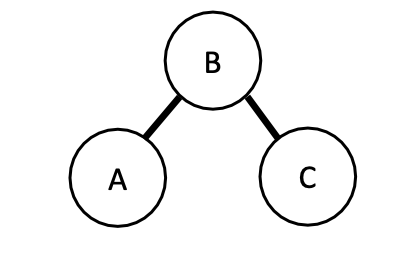
\includegraphics[width=0.3\textwidth]{p1.png}.
    \end{center}
    Give a 3 vertex in-order traversal and a 3 vertex pre-order traversal that cannot form a tree. That is, no single tree can have both the in-order traversal and the pre-order traversal.
    \begin{sol}
    \hspace*{\fill}\\
    in-order: ABC\\
    pre-order: CBA\\
    \textcolor{red}{    
    in-order: ABC\\
    pre-order: BCA}
    \end{sol}

    \item \ [6 pts] Using $n_0$ equal to 10, show that $f(n) = 7n^3 + 8n2 + 5n + 1 \text{ is } \Omega(n2)$.
    \begin{sol}
    \begin{align*}
        \Omega(g(n)) = \{f(n): & \text{ there exist positive constants } c \text{ and } n_0 \text{ such that } \\ 
       & 0 \leq cg(n) \leq f(n) \text{ for all } n \geq n_0\}\\
       & suppose \ g(n) = n^2\\
       & \therefore f(n) \geq cg(n)\\
       & 7n^3 + 8n^2 + 5n+1 \geq cn^2 \\
       & 7n + 8 + \frac{5}{n} + \frac{1}{n^2} \geq c \\
       & \lim_{n \to \infty} (7n + 8 + \frac{5}{n} + \frac{1}{n^2}) = \infty  \\
       & \because n_0 = 10 \\ 
       & \therefore \text{exit positive constants } 1 \text{ and } n_0, \\
       & let \ 7 \times 10 + 8 + \frac{5}{10} + \frac{1}{10^2} = 78.51 \geq 1 \\
       & \therefore f(n) = 7n^3 + 8n^2 + 5n + 1 \text{ is } \Omega(n^2)
    \end{align*}

    \textcolor{red}{
    \begin{align*}
        & 0 \leq c_1n^2 \leq 7n^3 + 8 n^2 + 5n+1, \forall \geq 10 \\
        & 0 \leq c_1 \leq 7n + 8 + \frac{5}{n}, \forall \geq 10 \\
        & c_1 \leq 70 \\
        & \text{Note that 70 is not a tight value, but works for the inequality.}
    \end{align*}
    }
    \end{sol}
    
    \item \ [8 pts] You run different programs for various values of ``n" and create 4 tables of the runtimes. Give the Asymptotic bounds that each of the tables support?
            \begin{center}
        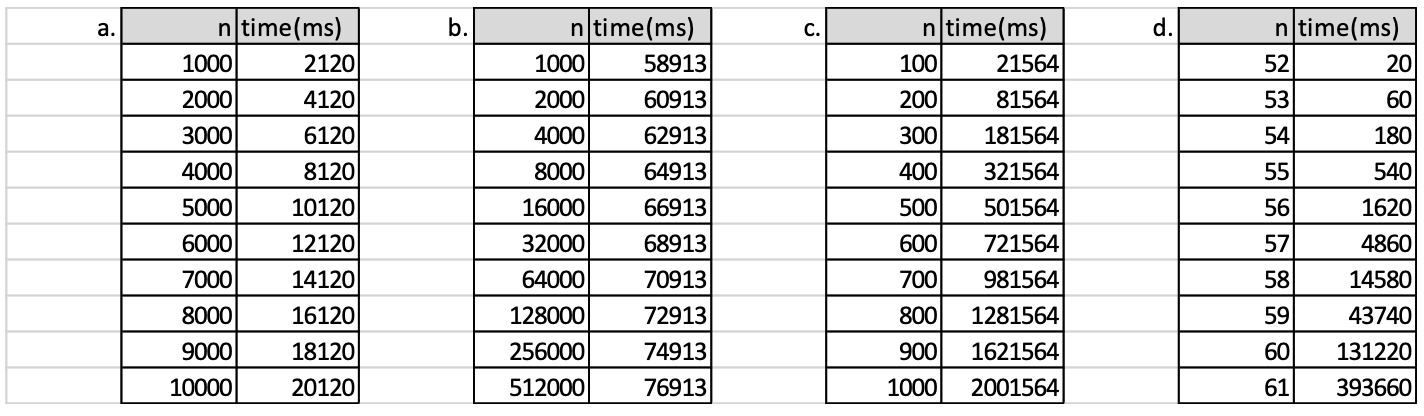
\includegraphics[width=0.9\textwidth]{p2.png}.
    \end{center}
    \begin{sol}
    \hspace*{\fill}
    \begin{enumerate}
        \item $\Theta(n)$
        \textcolor{red}{ \item $\Theta(\log_2(n))$}
        \item $\Theta(n^2)$
        \item $\Theta(3^n)$
    \end{enumerate}
    \end{sol}


    \item \ [6 pts] Answer the following Questions:
    \begin{enumerate}
        \item Given that $M > 100$ and $(7^{311} \bmod M ) = 1$; Find $7^{313} \bmod M =$ 
        \begin{sol}
            \textcolor{red}{49
            \begin{align*}
                & 7^{313} \bmod M = 7^{311+2} \bmod M = (7^{311} \bmod M) \times (7^2 \bmod M) = 49
            \end{align*}
            }
        \end{sol}
        \item Compute 1/3 mod 9 = 
        \begin{sol}
            Not exist.
        \end{sol}
        \item Compute $-\frac{1}{2} \bmod 11$
        \begin{sol}
        5
        \end{sol}
    \end{enumerate}

    % 8
    \item \ [8 pts] A message contains the following number of each symbol:\\
    \begin{align*}
            30 A’s, 14 B’s, 10 C's, 9 D's, 7 E's, 4 F's, 2 G's, 1 H \ and \ 1 \ K.
    \end{align*}
    Create a Huffman coding for each symbol:

    How many bits are in the entire Huffman coded message?
            \begin{sol}
        \hspace*{\fill}\\
        \begin{center}
        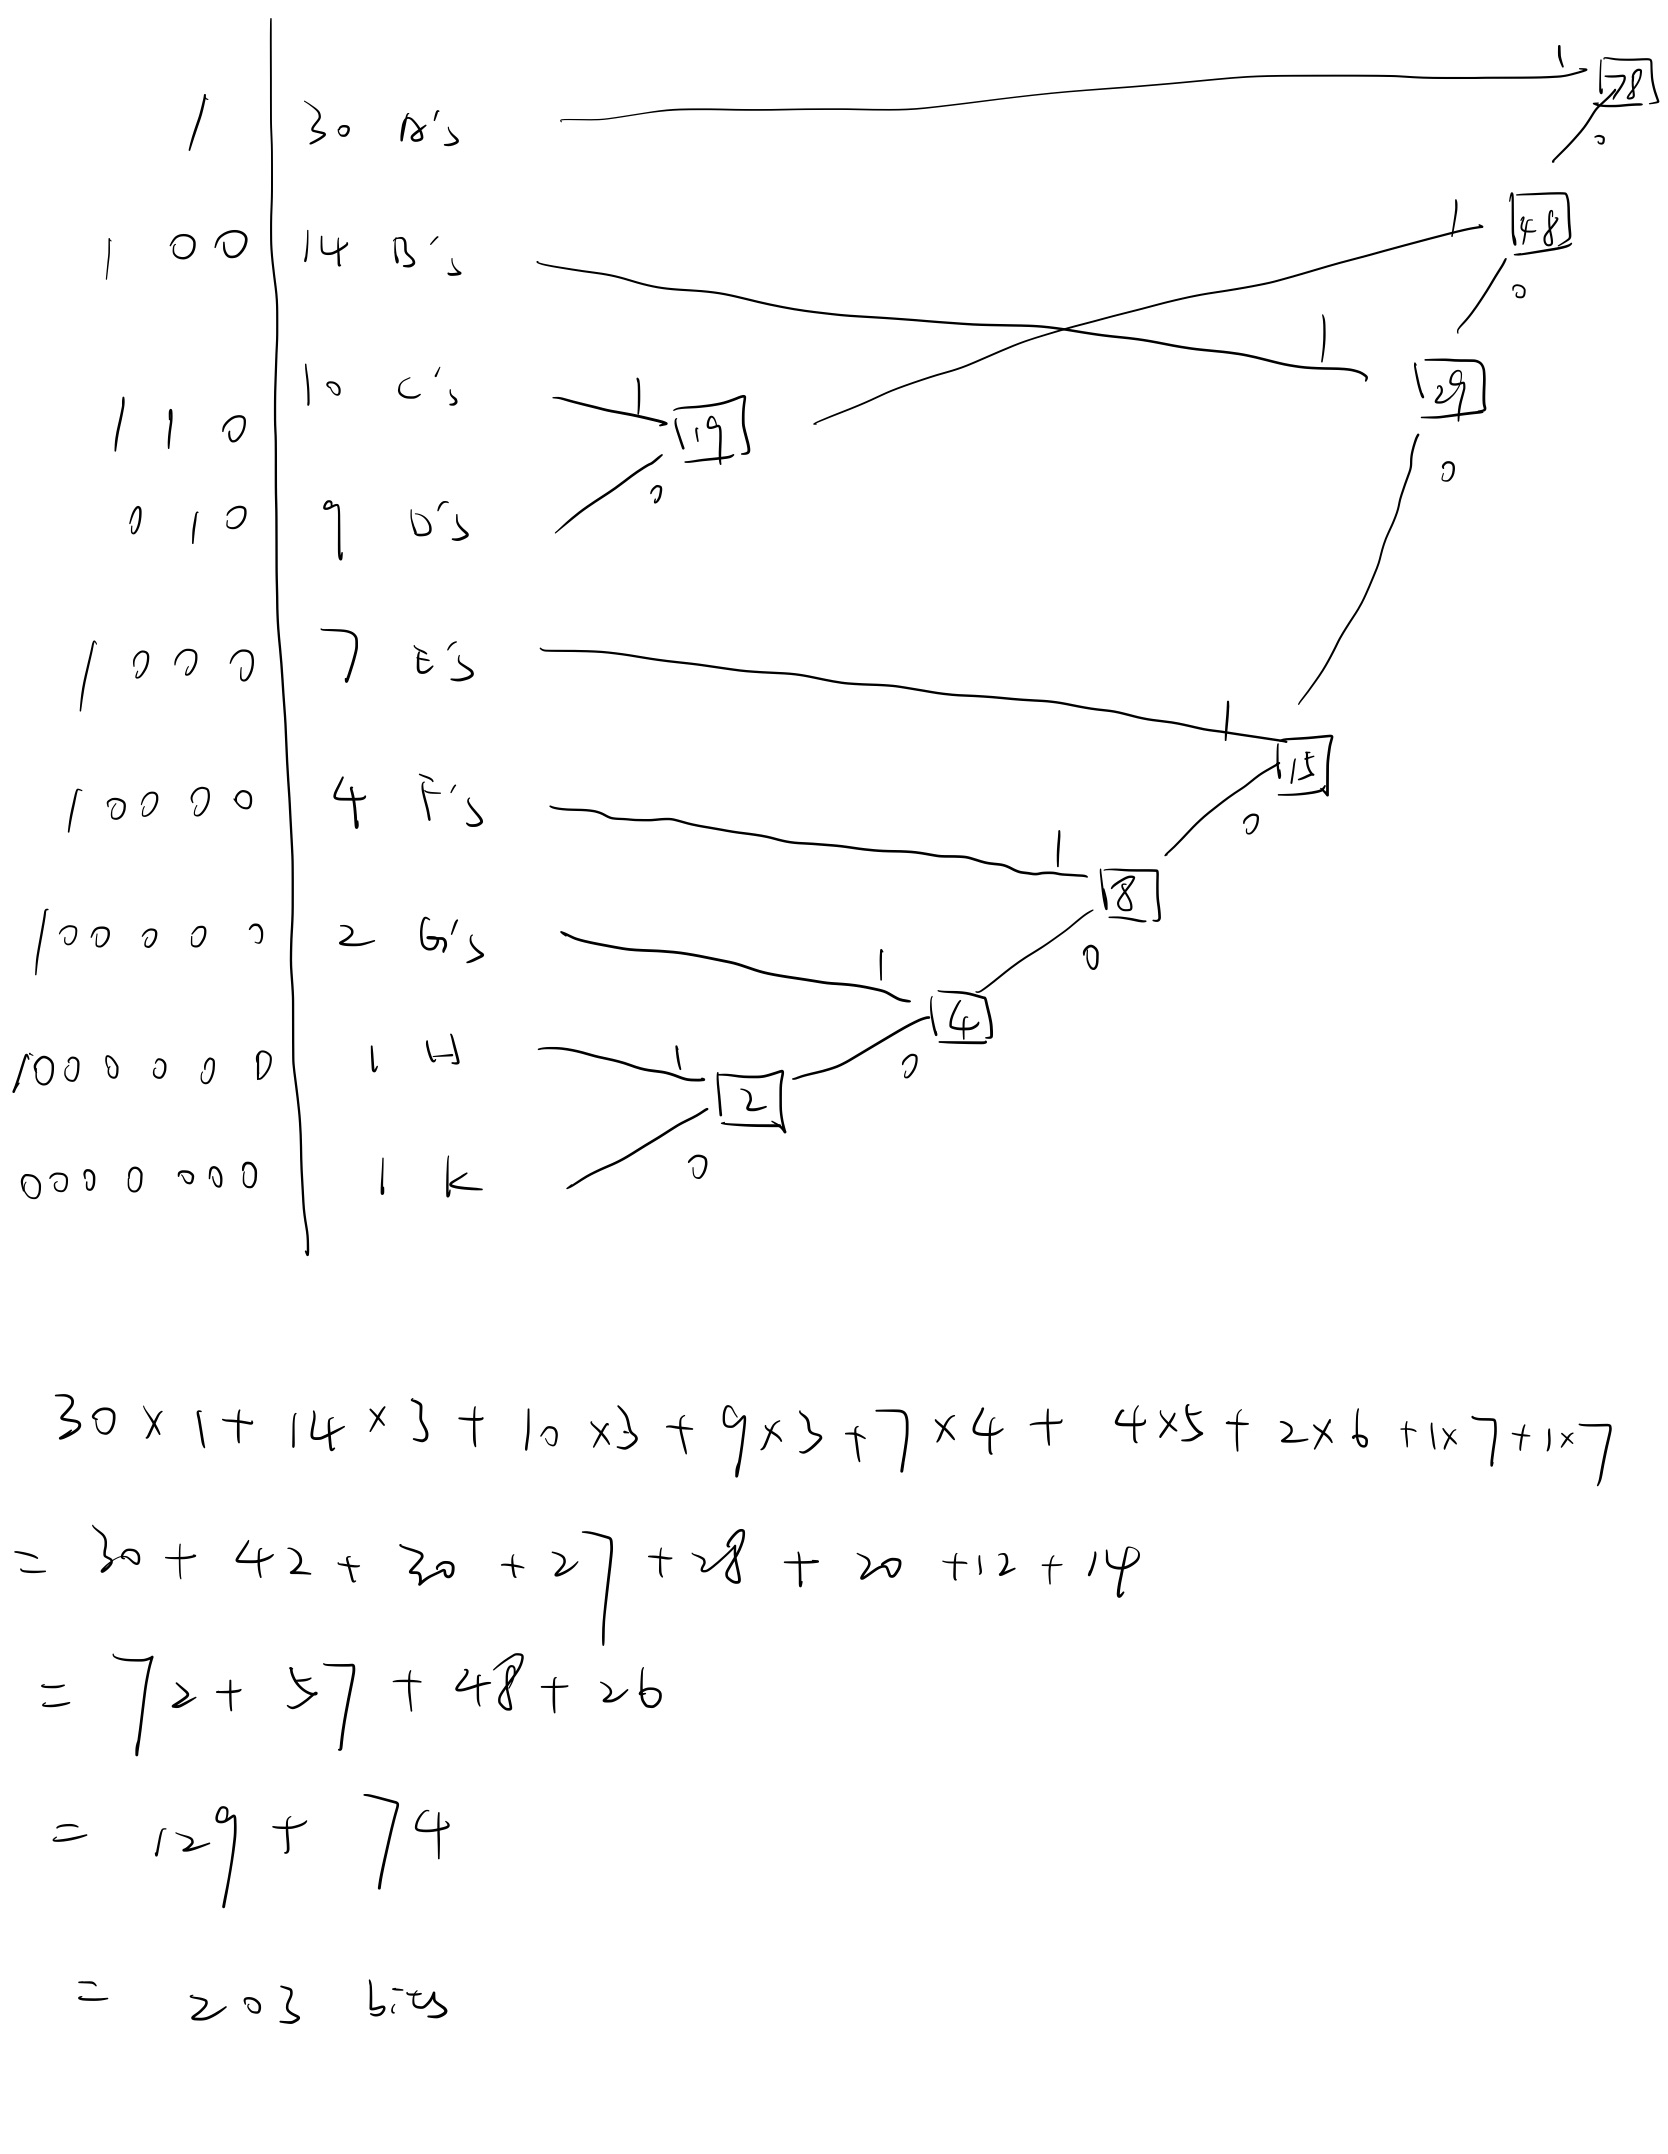
\includegraphics[width=0.9\textwidth]{p3.jpg}.
    \end{center}
        \textcolor{red}{203 bits}
        \end{sol}

    % 9
    \item \ [6 pts] Two people need to establish a secret key for encrypting communications. They agree to use a Diffie-Hellman key exchange with a modulus of 11 and decide on 2 as the base. Person A chooses a random value performs the appropriate computations and sends the value 3 to person B. Person B chooses a random value of 4 and performs the appropriate computations:
    \begin{enumerate}
        \item What is the value Person B sends to Person A
        \begin{sol}
            5
        \end{sol}
        \item What is the shared secret key between Person A and Person B
        \begin{sol}
            4
        \end{sol}

        \begin{sol}
        \hspace*{\fill}\\
        \begin{center}
        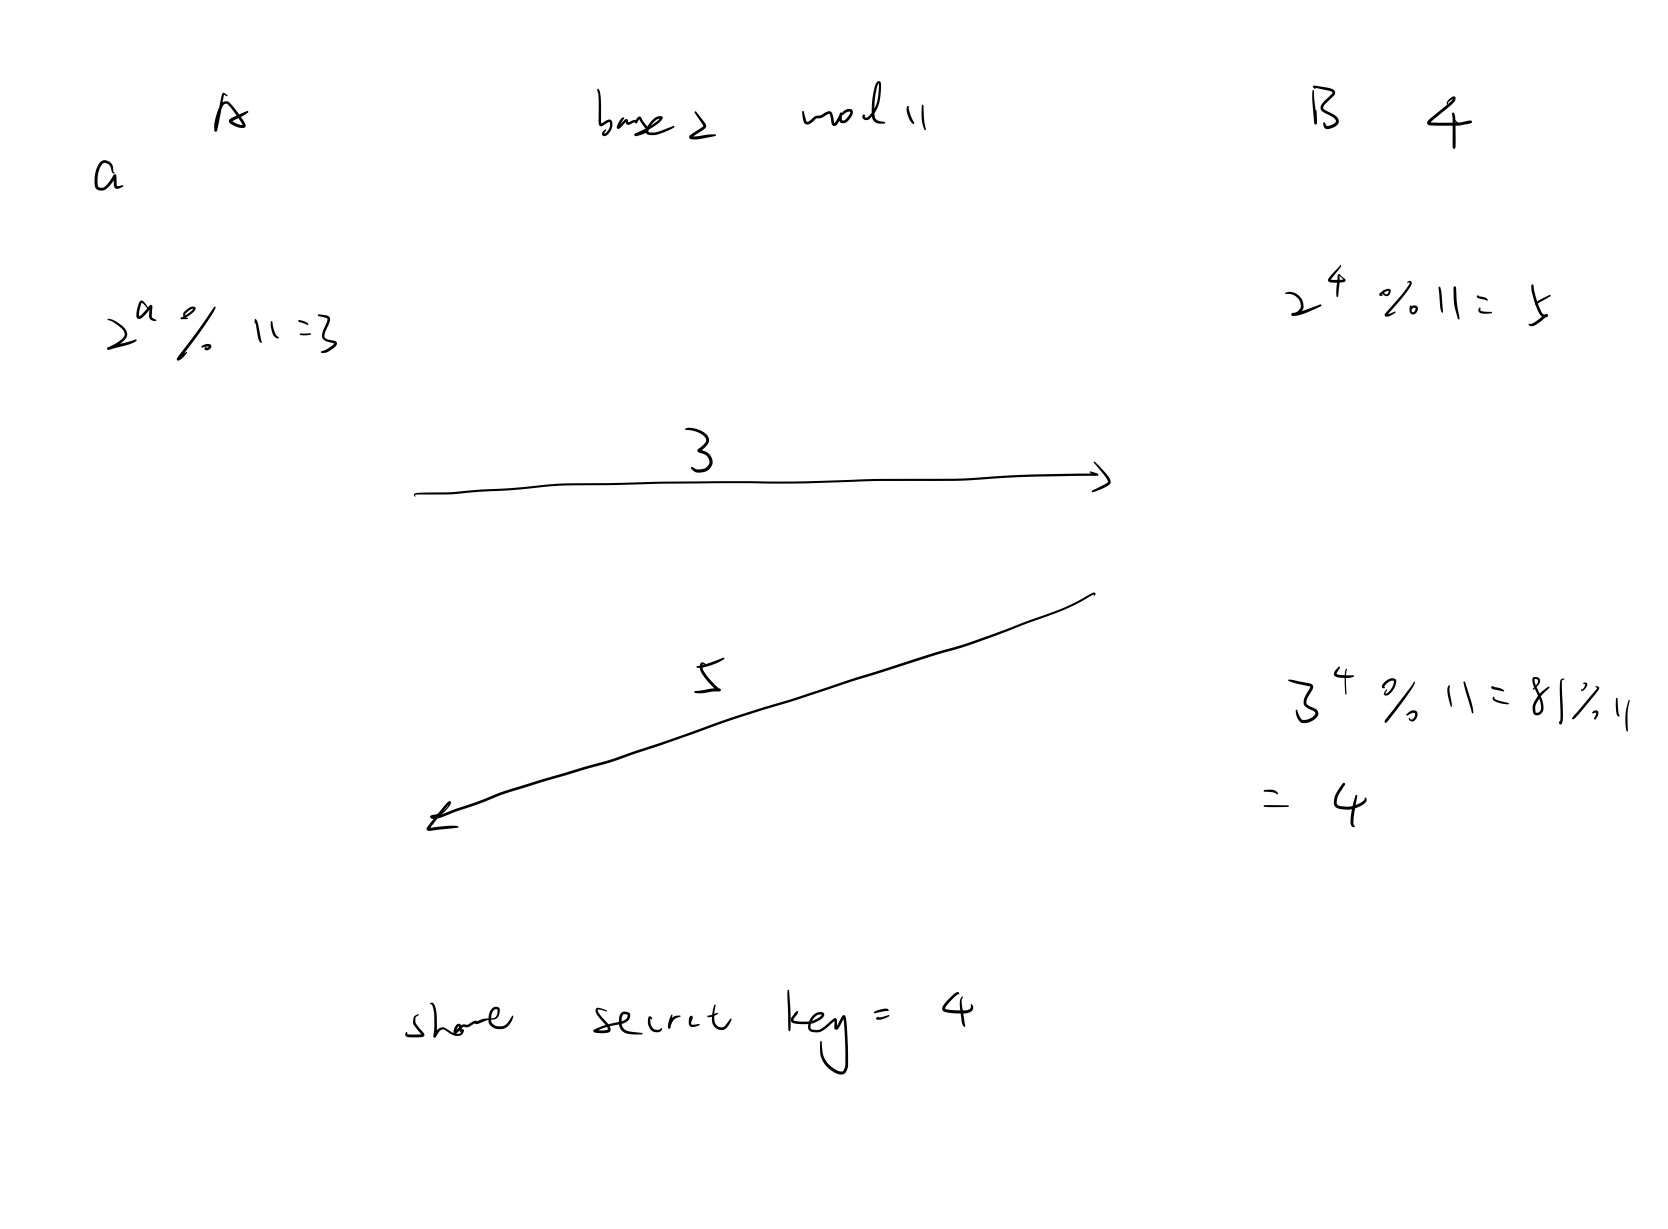
\includegraphics[width=0.9\textwidth]{p4.jpg}.
    \end{center}
        \end{sol}
    \end{enumerate}

    \item \ [9 pts] Consider two different algorithms that each solve a different problem.
    \begin{itemize}
        \item Implementation X solves Problem $P_x$ and Implementation X is $\Omega(n)$ and $O(n^2)$
        \item Implementation Y solves Problem $P_y$ and Implementation Y is $\Theta(2^n)$
    \end{itemize}
    Determine if each of these ``Yes it is true”,   ``Maybe it is true but doesn’t have to be”, or ``No it is not true”
    \begin{enumerate}
        \item Problem $P_x$ is harder than Problem $P_y$ : M
        \item Problem $P_y$ is harder than Problem $P_x$: M
        \item Implementation X is harder than Implementation Y: N
        \item Problem X is $\Omega(n)$: M
        \item Problem X is $\Omega(n^2)$: \textcolor{red}{M} %N
        \begin{sol}
            Problem x is $O()$ is between $O(n^2)$ and $\Omega(n)$
        \end{sol}
        \item Problem X is $O(n)$: \textcolor{red}{M} %N 
        \begin{sol}
                Problem x is $\Omega()$ is between $O(n^2)$ and $\Omega(n)$
        \end{sol}
        \item Problem X is $O (n^2)$: Y
        \item Implementation X is $\Omega(1)$: Y
        \item Implementation X is $O (2^n)$: Y

    \end{enumerate}


    \item \ [8 pts] The graph below represents containers that are transported between these cities each day. You are determining the maximum flow from vertex S, Vancouver, to vertex T, Winnipeg, using the Ford-Fulkerson algorithm in the graph below.
    \begin{center}
        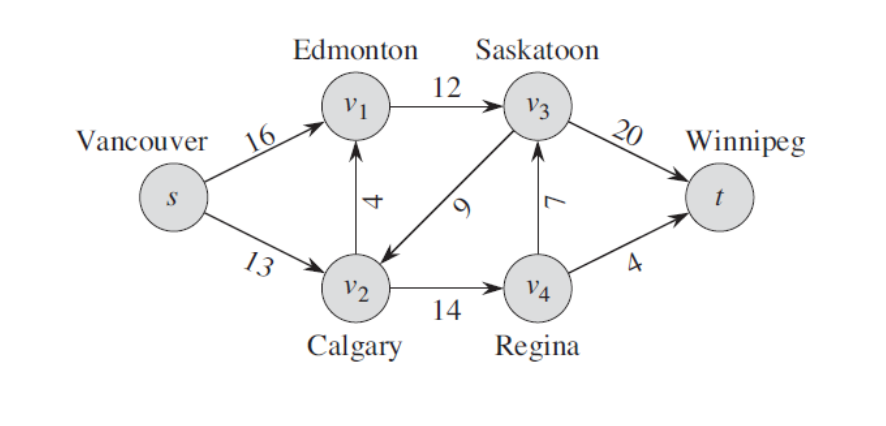
\includegraphics[width=0.8\textwidth]{p5.png}.
    \end{center}
    A Path Search finds the path $s \rightarrow v2 \rightarrow v4 \rightarrow v3 \rightarrow t$.
    \begin{enumerate}
        \item How much flow is in this path?
        \begin{sol}
            7
        \end{sol}
        \item What does the new graph look like after “removing” this flow
        \begin{sol}
                \begin{center}
        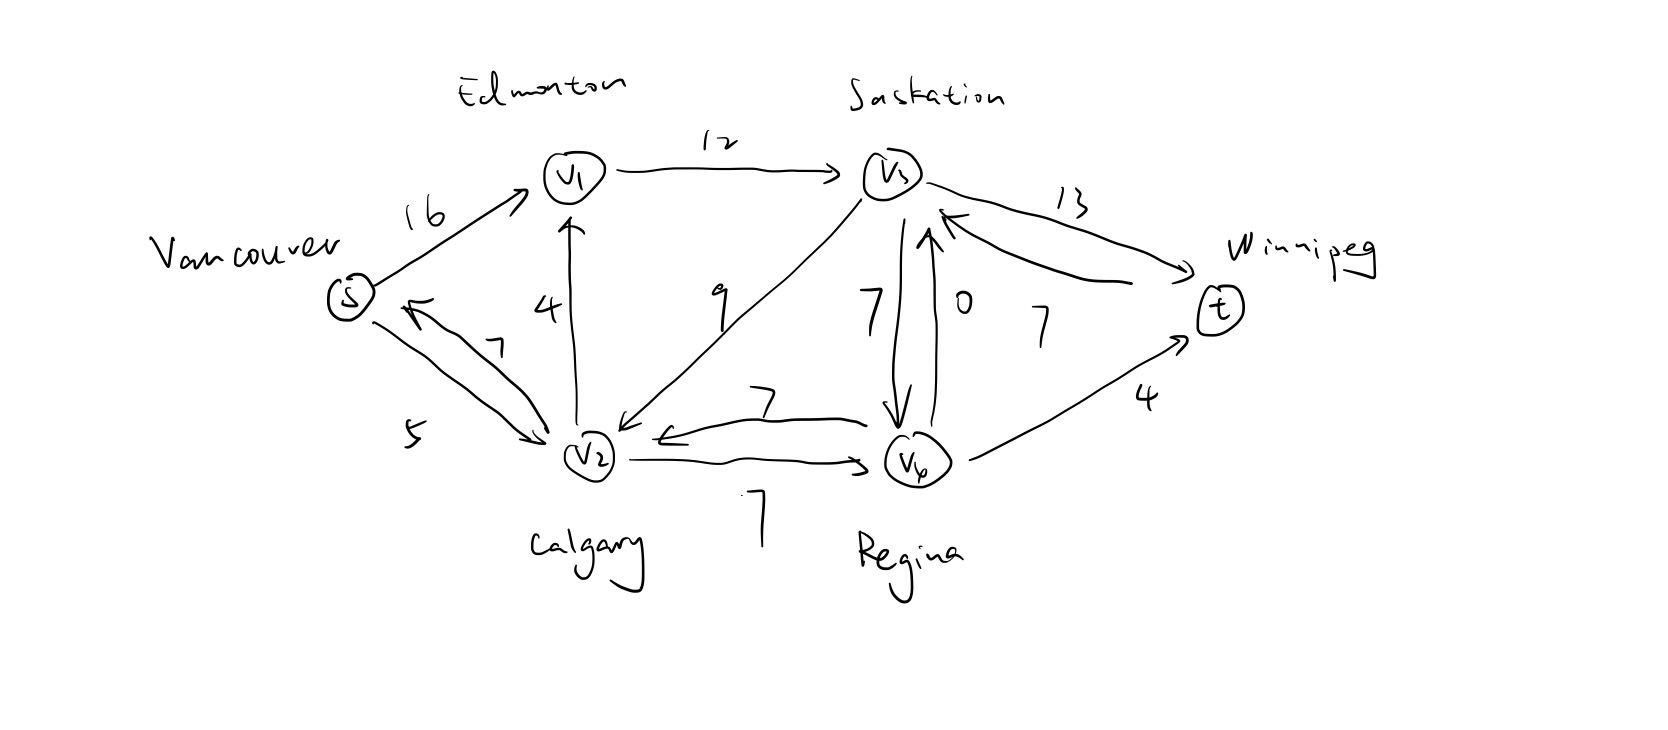
\includegraphics[width=0.8\textwidth]{p6.jpg}.
    \end{center}
        \end{sol}
            A Path Search now finds the path $s \rightarrow v1 \rightarrow v3 \rightarrow v4 \rightarrow t$ on the new graph.
            \item Is it possible to find this path?
            \begin{sol}
                Yes
            \end{sol}
            \item If so, how much flow is in this path?
            \begin{sol}
                4
            \end{sol}
    \end{enumerate}

    \item \ [10 pts] Answer the following questions.:
        \begin{enumerate}
            \item A program requires 6 seconds to process an input size of 40. If the running time is $\Theta(\sqrt(n))$ about how large of an input set could you process in 160 seconds?
            \begin{sol}
            \begin{align*}
                \frac{\sqrt{n}}{\sqrt{40}} \times 6 = 160 \rightarrow n \approx 28445
            \end{align*}
            \end{sol}

            \textcolor{red}{\item A program requires 2 DAYS to brute force attack a password of 64 bits. Since the running time is $\Theta(2^n)$ about how MANY DAYS would it take for the program to brute force attack a password of 256 bits?}
            \begin{sol}
            \begin{align*}
                \frac{2^{256}}{2^{64}} \times 2 = 2^{192} \times 2 = 2^{193} \ days
            \end{align*}
            \end{sol}

            \textcolor{red}{\item A program requires 2 DAYS to brute force attack a password of 64 bits. About how MANY DAYS would it take for the program to brute force attack a password of 256 bits if the running time were $\Theta(n^2)$ instead of exponential?}
            \begin{sol}
                \begin{align*}
                    \frac{256^2}{64^2} \times 2 = 16 \times 2 = 32 \ days
                \end{align*}
            \end{sol}

            \item A program requires 4 milliseconds to process an input size of 1000. If the running time is $\Theta(n^4)$ about how many seconds would it take to process an input size of 1 million items?
            \begin{sol}
                \begin{align*}
                    \frac{n^4}{1000^4} \times 4 \times 10^{-3} \ seconds = (\frac{10^6}{10^3})^4 \times 10^{-3} = 4 \times 10^9 \ seconds 
                \end{align*}
            \end{sol}

            \item A program requires 4 milliseconds to process an input size of 1000. If the running time is $\Theta(n)$ about how long many seconds will it take to process an input size of 1 million items?
            \begin{sol}
                            \begin{sol}
                \begin{align*}
                    \frac{n}{1000} \times 4 \times 10^{-3} \ seconds = (\frac{10^6}{10^3}) \times 4 \times 10^{-3} = 4 \  seconds 
                \end{align*}
            \end{sol}
            \end{sol}
        \end{enumerate} 

        \item \  [5 pts] You live in city B. You want to know the cost to travel from city B to all other cities (A,B,C,D,E,F,H and I). The edges of the graph below represent the cost to travel the roads between various cities. If an edge doesn’t exist, then there is no road between those two cities.
        \begin{center}
        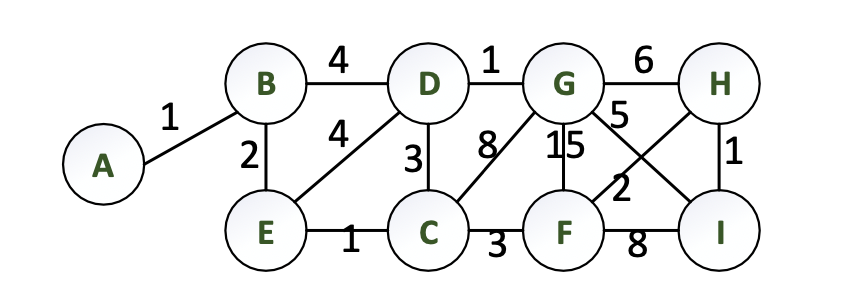
\includegraphics[width=0.5\textwidth]{p7.png}.
         \end{center}
         What is the order in which you explore the cities using Dijkstra’s Single Source
Shortest Path algorithm to find the cost from city B to all other cities in the graph?
        \begin{sol}
        \hspace{\fill}\\
                    \begin{center}
        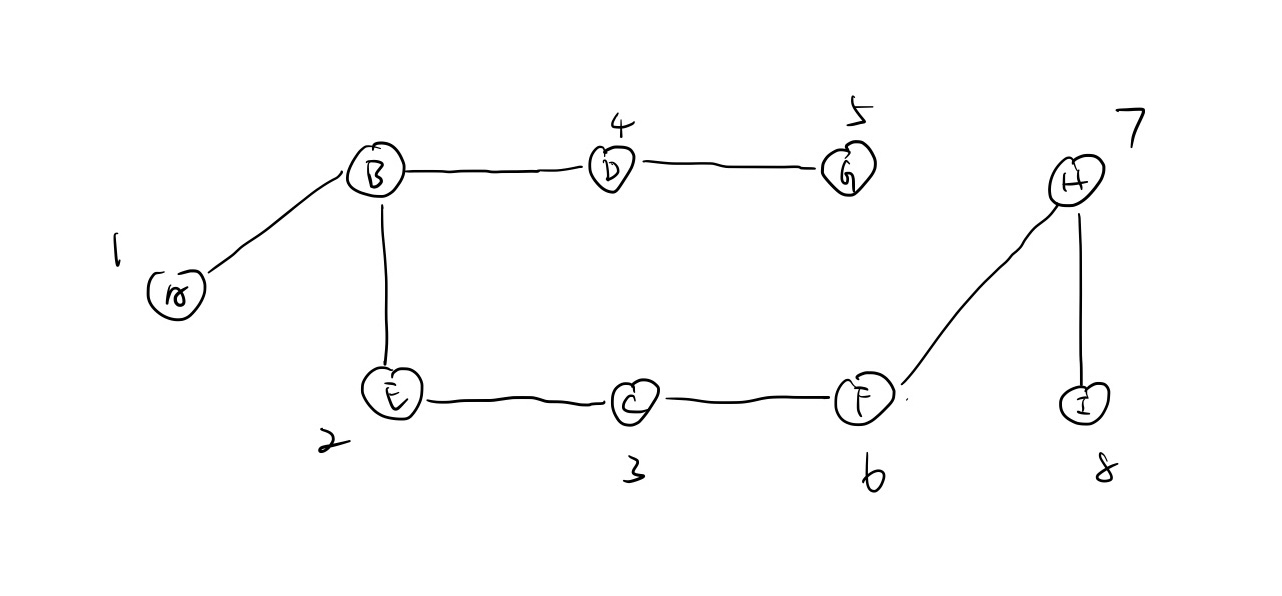
\includegraphics[width=0.9\textwidth]{p8.jpg}.
        
         \end{center}
         \textcolor{red}{BAECDGFHI}
        \end{sol}

        \item \  [5 pts] Give a smallest last vertex ordering for the graph in Problem \#13. Circle in your ordering the first vertex you wrote down for that ordering.
                            \begin{center}
        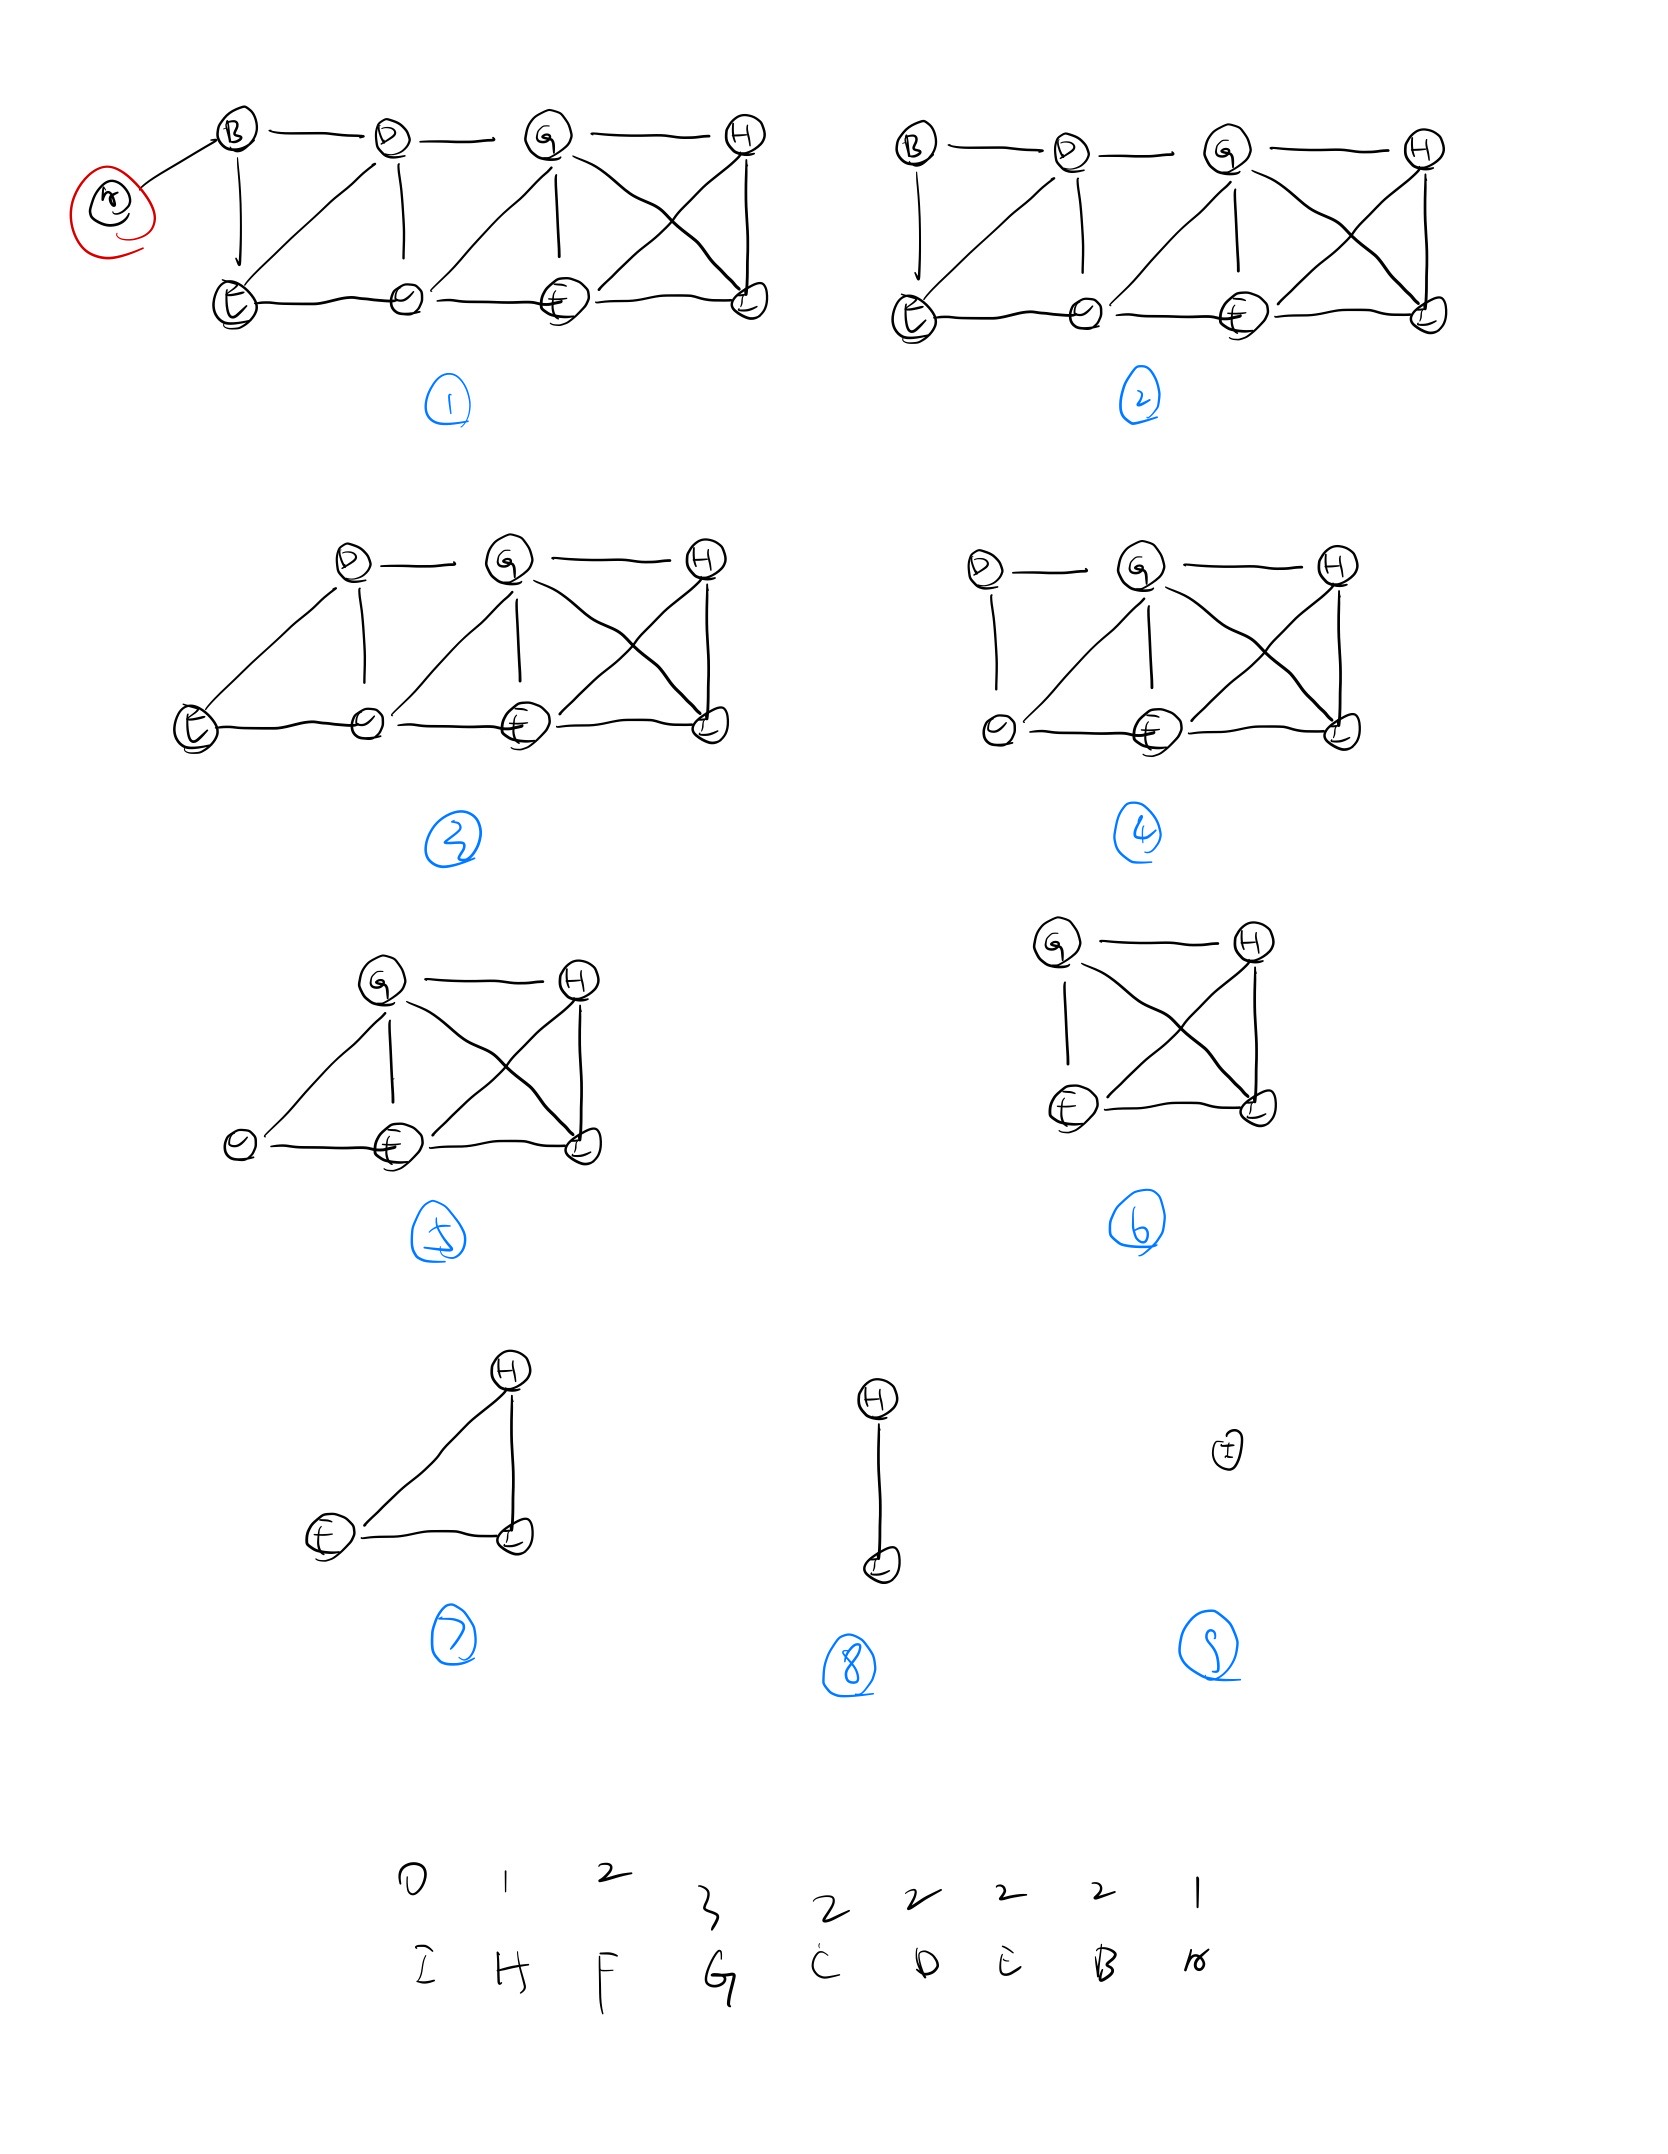
\includegraphics[width=0.9\textwidth]{p9.JPG}.
        \end{center}
\end{enumerate}

\end{document}
